Since the mid-1980s, the US labour share fell considerably. Figure \ref{fig:labour_shares} shows a clear downward trend for four measures of the labour share after 1987 \footnote{Section \ref{sec:data} discusses the four methods I use to measure the labour share.}. A large macroeconomic literature has attempted to uncover the mechanisms driving the shift in the distribution of income away from labour, yet no clear consensus has been reached.


\begin{figure}[h]
    \centering
    \caption{\normalsize Aggregate labour share decline relative to 1987, percentage point change}
    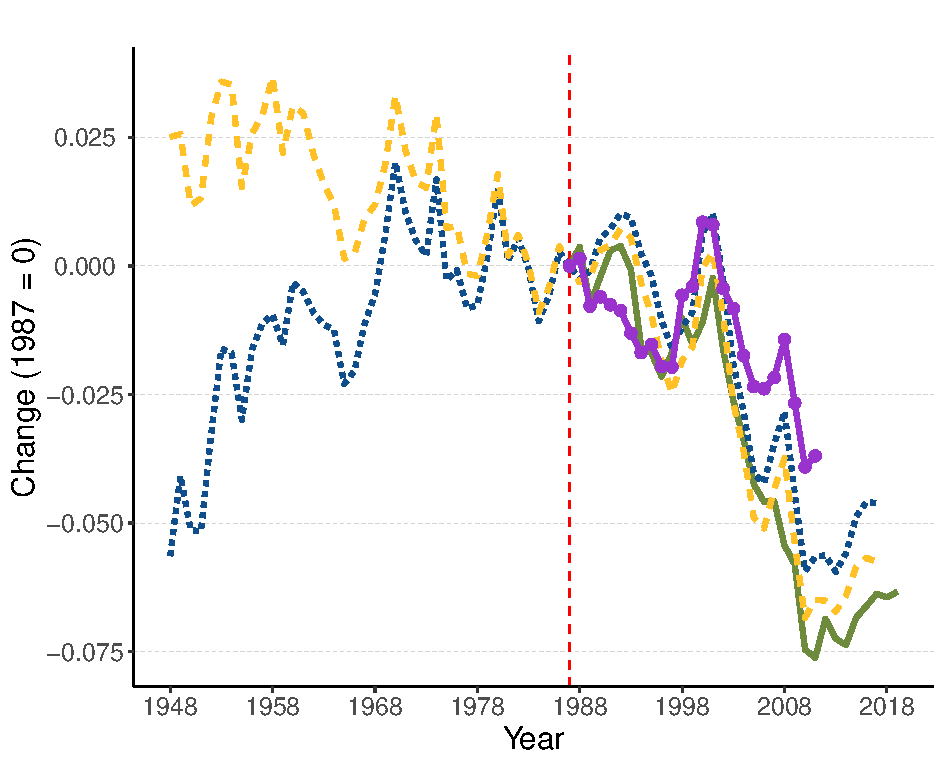
\includegraphics[width=10cm]{Introduction/diff_labour_shares.pdf}

    \label{fig:labour_shares}

\begin{minipage}{\linewidth}
    \caption*{\textit{Notes}: The aggregate labour share equals labour income (self-employed labour income + payroll labour income) divided by GDP. The labour income of self-employed individuals is imputed four different ways. Section \ref{sec:data} contains the data description. \\
    \textit{Source}: Bureau of Economic Analysis (BEA), Bureau of Labour Statistics (BLS), and author's calculations.}
\end{minipage}
\end{figure}

\noindent The decline in the labour share coincided with a substantial reallocation of value-added towards sectors with high labour share levels, mainly in services \citep{boppartStructuralChangeKaldor2014, herrendorfTwoPerspectivesPreferences2013, gagglStructuralChangeProduction2023, bridgmanLaborShareMarkups2023}. All else equal, such reallocation should counterfactually raise the labour share, as the aggregate reflects the higher labour shares in the growing sectors to a greater extent. How much of the declining labour share is due to reallocation between sectors with different labour share levels and how much arises due to labour shares changing within sectors? 

Despite the reallocation towards industries with high labour shares, numerous studies, including \citet{daoWhyLabourReceiving2019a, elsbyDeclineLaborShare2013a} and \citet{karabarbounisGlobalDeclineLabor2014a}, argue that between-sector compositional changes do not play a role in the decline of the US labour share, so aggregate movements should be understood primarily as a within-sector phenomenon. In this paper, I show that the apparent lack of a reallocation effect is due to the specific decomposition method used in previous studies. First, I theoretically compare the commonly used shift-share (between-within) decomposition to the \citet{haltiwangerMeasuringAnalyzingAggregate1997} (between-within-cross) decomposition (henceforth, I refer to it as the `Haltiwanger decomposition'). The two methods are closely related because they both decompose the same change in the aggregate labour share. However, the additional cross term in the Haltiwanger decomposition explicitly captures the impact of covarying sectoral weights (relative size) and sectoral labour shares on the aggregate labour share. I theoretically show the shift-share between- and within-sector contributions include half of the Haltiwanger cross term. Therefore, the shift-share decomposition unintentionally counts half of the covariance impact as between-sector reallocation. The same holds for the within-sector contribution. 

% Specifically in the US context, 

% Adjusting for the effect of the covariance is important in the US context in which the reallocation towards high labour share sectors interacts with sector-specific levels and trends in labour shares.  

% The reallocation effect is missing in previous studies by virtue of the decomposition method used. 

Second, I show the cross contribution is large and negative using US industry data and four different measures of the labour share. Following my theoretical result, the between- and within-sector contributions measured using the shift-share decomposition are downward biased because half of the negative covariance is added to each. Decomposing the declining payroll labour share using the shift-share method attributes only 4\% to reallocation and the remaining 96\% to within-sector mechanisms. A shift-share decomposition implies that to explain the path of the aggregate labour share one needs only to examine the determinants of labour shares within sectors. However, using the Haltiwanger decomposition - which removes the impact of co-movement between sectoral weights and sectoral labour shares - reallocation accounts for -47\% of the total decline. The Haltiwanger decomposition recovers the positive reallocation effect missing from previous studies. In addition, the impact of within-sector mechanisms falls from 96\% to 45\% when using the Haltiwanger decomposition. I find similar results for three other measures of the aggregate labour share. The Haltiwanger decomposition highlights the quantitative importance of three channels operating in tandem to depress the labour share: reallocation towards industries with high labour share levels, declining labour shares within sectors, and the negative co-movement between sectoral weights and sectoral labour shares. 

% need 'missing reallocaion effect' here
% need to talk about the size of the cross term
% need to talk about the three channels emerging 

 
 % THE NEW THING IS THAT CROSS TERMS ARE ALSO IMPORTANT ---> EXPLAINING 100\% OF THE DECLINE WHILE THE OTHER TWO CANCEL OUT... ALSO MENTION THE SELF-EMPLOYED 

\vspace{0.3cm}

\textbf{Related Literature.} The negligible reallocation effect found in previous studies leads to authors proposing within-sector mechanisms to explain the falling labour share. Falling sectoral labour shares are related to the increased adoption of automation \citep{acemogluAutomationNewTasks2019}, rising concentration \citep{barkaiDecliningLaborCapital2020}, intermediate inputs prices \citep{castro-vincenziIntermediateInputPrices2022}, and sectoral heterogeneity in trade exposure \citep{elsbyDeclineLaborShare2013a}. Why these mechanisms would not also cause reallocation between sectors is not clear. For instance, increased trade exposure with China displaced manufacturing employment and automation is likely to promote growth heterogeneously across sectors that benefit differently from its adoption \citep{autorChinaSyndromeLocal2013, acemogluAutomationNewTasks2019}. Since I find that reallocation and co-movements between sectors' size and labour shares are also important channels affecting the aggregate labour share, a methodology flexible enough to accommodate both is necessary to parse out which of the above mechanisms is driving the decline in the labour share. 

% that to parse out which factors are quantitatively important, a methodology flexible enough to incorporate the effect of each on reallocation between sectors, and, hence, co-movements between sectors' size and labour shares, is necessary. 


% While not ruling any of the literature's proposed mechanisms out, my findings suggest a unified framework incorporating reallocation and, hence, co-movements between sectors' size and labour shares can more richly explain the underlying dynamics of the aggregate labour share.

% need to talk about using frameworks that examine the same factors but allow for the reallocation effect to be measured... 

\citet{bridgmanLaborShareMarkups2023} and \citet{feijomoreiraDeclineLaborShare2022} find a positive reallocation effect on the aggregate labour share in two-sector structural models. However, neither paper explains why their results differ from previous seminal studies claiming reallocation has no effect. My paper bridges this gap.

Lastly, \citet{autorFallLaborShare2020} and \citet{kehrigMicroLevelAnatomyLabor2021a} decompose changes in sectoral labour shares at the establishment level using US Census data. The authors explicitly measure the impact of co-movement between establishments' size (reallocation) and their labour shares on different industries' labour shares. Both papers find that co-movements drive sectoral trends. The establishment-level data allows for a more granular analysis than the industry-level data I use. However, the establishment-level data is not consistently measured across sectors, whereas the industry-level data covers the entire economy. 

% Because robust firm-level measures of value added are not avail- able from the Economic Census outside of manufacturing, we use the cruder measure of the ratio of payroll to sales. 

% it does not afford a comprehensive view of 

% the data does not cover the entire economy, coverage is not consistent and comprehensive 

% leads to a more granular analysis, but is not comprehensively cover the entire economy (consistently) 

% the authors are not able to examine the labour share of the entire economy 

% means the authors cannot examine the labour share of the entire economy. In contrast, the detailed industry-level data I use covers the entire economy. 


% The difference is made up by the large and negative cross term, which accounts for 103\% of the aggregate decline. 

% * and mention replication of previous Elsby study

% use between-within (shift-share) decompositions and claim between-sector reallocation does not offset the fall in the labour share. As a result, the authors of these papers only examine within-sector mechanisms as potential drivers of the labour share, for example by regressing sectoral trade exposure and the adoption of automation on changes in sectoral labour shares. First, it is unclear why these mechanisms would not also cause reallocation between sectors. For instance, increased trade exposure displaces manufacturing employment and automation is likely to promote growth heterogeneously across sectors that benefit differently from its adoption \citep{autorChinaSyndromeLocal2013, acemogluAutomationNewTasks2019}. Second, given the clear reallocation we see towards high labour share sectors, why is the reallocation effect missing from the results in the literature? 

% To bridge the gap, I exploit the between-within-cross decomposition from \citet{haltiwangerMeasuringAnalyzingAggregate1997}, rather than the between-within decomposition used in all previous studies in the literature. The additional cross term in the Haltiwanger decomposition explicitly accounts for co-movements in between-sector and within-sector mechanisms, which is important in the US context where reallocation coincides with sector-specific trends affecting the labour share within sectors. In the between-within decomposition, the effect coming from co-movement is split evenly across the between-sector and within-sector terms. As a result, the between-sector term, which is meant to capture the impact of reallocation, is also capturing the impact of co-movements. Using the between-within-cross decomposition, reallocation accounts for -47\% of the decline in the aggregate payroll labour share (the percentage is negative because reallocation offsets the decline). Using the between-within decomposition, reallocation accounts for 4\% of the decline, an order of magnitude smaller. The reason the results change so dramatically is the additional cross term in the Haltiwanger decomposition is large and negative and cancels out the positive between-sector effect in the between-within decomposition. Furthermore, reallocation accounts for a similar portion of the decline when accounting for self-employed individuals' labour income as well. 

% My results imply the missing reallocation effect is an artefact of the decomposition method used in previous studies. Therefore, to understand the falling labour share an integrated approach combining between-sector reallocation, within-sector mechanisms, and co-movements of the two is needed. Previous models attempting to explain the decline often ignore the notion of a sector's size and, therefore, cannot account for the reallocation channel. While not the goal of this paper, my results provide realistic calibration targets for models of the declining labour share incorporating all three channels. Furthermore, \citet{grossmanElusiveExplanationDeclining2022} argue the falling labour share has been explained ``many times over'' by the literature, due to the focus only on factors leading to its decline. My results help to partly reconcile their point because reallocation partially offsets the decline. 

 % \citet{elsbyDeclineLaborShare2013a, barkaiDecliningLaborCapital2020, daoWhyLabourReceiving2019a, castro-vincenziIntermediateInputPrices2022, acemogluAutomationNewTasks2019} and \citet{karabarbounisGlobalDeclineLabor2014a} all propose various within-sector mechanisms to explain the fall in the labour share. Examples include regressing sectoral trade exposure, adoption of automation, rising concentration, and rising intermediate input prices on labour shares within sectors. The reason they examine mechanisms at the sectoral level is standard shift-share decompositions measure the effect of reallocation to be negligible. First, the proposed mechanisms are also likely to lead to reallocation between sectors, as mentioned before. Second, my results indicate reallocation is also a relevant channel for the aggregate labour share, and, therefore, should also be incorporated. In this way, my paper complements the pre-existing literature. 

